\chapter{Introdução à análise sintática}

\section{Introdução}

Após a análise léxica, o programa de entrada foi convertido em uma
lista de tokens. O próximo passo da compilação é a análise sintática,
também chamada de \textbf{parsing}, na qual o compilador verifica se
os tokens formam uma sintaxe válida da linguagem. Para além de uma
resposta booleana, analisadores sintáticos constroem uma
representação do programa como uma árvore para uma uso em fases
posteriores do compilador.

É importante ressaltar que o analisador sintático não realiza todas
as verificações restantes sobre o programa; por exemplo, não é
responsabilidade do analisador sintático determinar se tipos são
compatíveis ou se todas as variáveis estão declaradas. Essas
verificações são feitas em outra etapa, a análise semântica.

A análise sintática é um tópico bem estabelecido na ciência da
computação e seu estudo pode fornecer ideias para aplicações em
outras áreas visto que não apenas compiladores precisam analisar informações.

\section{Gramáticas livres de contexto}

Neste curso, adotamos a abordagem de construir implementações a
partir de especificações precisas. Como podemos especificar a sintaxe
válida de programas em uma linguagem de programação? Vimos que, para
o problema de especificar tokens válidos, as expressões regulares nos
fornecem uma linguagem de especificação suficientemente expressiva.
Infelizmente, as expressões regulares não são suficientes para
representar a sintaxe da maioria das linguagens de programação.

Uma maneira fácil de perceber isso é considerar a necessidade de
verificar se os parênteses e outras construções de agrupamento estão
devidamente balanceados. Para balancear os parênteses, é necessário
contar o número de parênteses abertos que ainda não foram fechados.
No entanto, as expressões regulares podem ser reconhecidas por
autômatos finitos, enquanto que contar um número ilimitado de
parênteses exigiria um número ilimitado de estados. Nenhum autômato
finito consegue controlar o número de parênteses desbalanceados,
portanto, as expressões regulares não são suficientemente poderosas
para especificar a sintaxe da linguagem.

Essa limitação das expressões regulares motiva o uso de gramáticas
livres de contexto (GLCs) para especificar a sintaxe da linguagem.

Uma gramática livre de contexto é caracterizada por um conjunto de
produções. Cada produção explica como reescrever um símbolo não
terminal em alguma sequência de símbolos terminais (tokens) ou
símbolos não terminais. Como exemplo, temos a seguir uma gramática
para uma linguagem de expressões aritméticas:

\[
  \begin{array}{lclclclcl}
    E & \to & n & | & E + E & | & E * E & | & (E)
  \end{array}
\]

em que \(\Sigma=\{+,*,(,),n\}\) são \textbf{tokens} desta linguagem.

Dada uma gramática \(G = (V,\Sigma, R, P)\), uma palavra pertence à
sua linguagem, \(L(G)\), se existir alguma derivação desta string
usando as regras de \(G\). Uma derivação é uma sequência de
reescritas que começa com a variável inicial e eventualmente termina
na palavra considerada. Cada passo na sequência aplica alguma
produção da gramática: realiza uma reescrita \[
  \alpha A \beta \to \alpha \gamma \beta
\] em que \(A \to \gamma\) é uma regra de \(G\).

Por exemplo, a palavra \haskell{(1+4)+2} pertence à
linguagem da gramática. Podemos verificar isso construindo uma derivação: \[
  \begin{array}{lc}
    E     & \Rightarrow \\
    E + E & \Rightarrow\\
    (E) + E & \Rightarrow\\
    (E + E) + E & \Rightarrow \\
    (1 + E) + E & \Rightarrow \\
    (1 + 4) + E & \Rightarrow\\
    (1 + 4) + 2
  \end{array}
\] Essa derivação é uma derivação mais à esquerda: a cada passo, o
não terminal expandido é o não terminal mais à esquerda. Como veremos
em breve, as derivações mais à esquerda são construídas por
analisadores sintáticos descendentes. Também é possível construir uma
derivação mais à direita para qualquer string, expandindo o não
terminal mais à direita a cada passo. Por exemplo, a derivação mais à
direita da mesma string procede da seguinte forma: \[
  \begin{array}{lc}
    E     & \Rightarrow \\
    E + E & \Rightarrow\\
    E + 2 & \Rightarrow\\
    (E) + 2 & \Rightarrow \\
    (E + E) + 2 & \Rightarrow \\
    (E + 4) + 2 & \Rightarrow\\
    (1 + 4) + 2
  \end{array}
\]

Uma derivação corresponde a uma árvore sintática, na qual a raiz é o
símbolo inicial e as folhas foram a string do programa processado.
Ambas as derivações acima correspondem à seguinte árvore de análise sintática:

\begin{figure}[H]
  [
    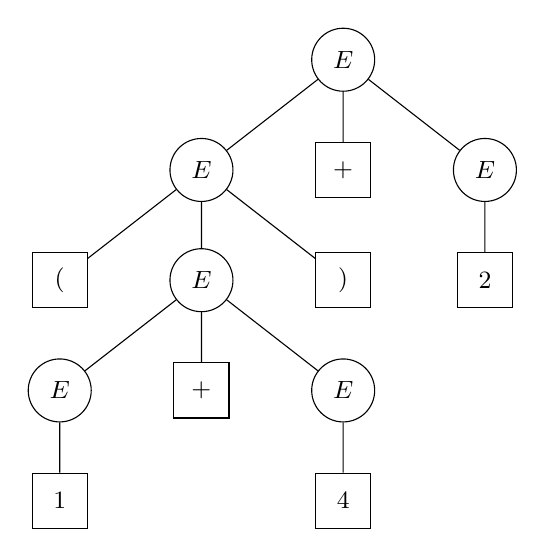
\begin{tikzpicture}[
        level distance=1.4cm,
        sibling distance=1.8cm,
        every node/.style={font=\small},
        every child/.style={edge from parent/.style={draw}},
        nonterminal/.style={circle, draw, minimum size=8mm},
        terminal/.style={rectangle, draw, minimum size=7mm,
        font=\small\bfseries},
      ]

      \node[nonterminal] {$E$}
      child { node[nonterminal] {$E$}
        child { node[terminal] {$($} }
          child { node[nonterminal] {$E$}
            child { node[nonterminal] {$E$}
              child { node[terminal] {$1$} }
            }
            child { node[terminal] {$+$} }
            child { node[nonterminal] {$E$}
              child { node[terminal] {$4$} }
            }
          }
        child { node[terminal] {$)$} }
      }
      child { node[terminal] {$+$} }
      child { node[nonterminal] {$E$}
        child { node[terminal] {$2$} }
      };

    \end{tikzpicture}
    \centering
  \end{figure}

  Embora essas duas derivações gerem a mesma árvore de análise
  sintática, é possível, em geral, que uma string tenha mais de uma
  árvore sintática. Quando isso acontece, diz-se que a gramática é
  ambígua. Uma gramática ambígua é aquela para a qual existe alguma
  string com múltiplas árvores sintáticas.

  Nossa gramática de exemplo é, de fato, ambígua. Por exemplo,
  considere a string \haskell{2 + 3 * 4}. Ela possui
  uma árvore de análise sintática na qual a produção \(E \to E + E\) é
  usada na raiz, mas também outra árvore na qual a produção \(E \to E *
  E\) é usada na raiz. Considerando-as como expressões aritméticas, a
  primeira árvore de análise sintática corresponde ao valor esperado da
  expressão, 14. A segunda árvore de análise sintática corresponde ao
  cálculo de 20: possivelmente, a resposta errada. O problema com a
  gramática é que ela não impõe precedência ou associatividade aos
  operadores + e *.

  \subsection{Representando precedência e associatividade}

  Garantir precedência e associatividade é um problema comum no projeto
  de gramáticas. Felizmente, existem algumas maneiras padronizadas de
  lidar com isso.

  O problema com a gramática original é que ela permite que a produção
  \(E \to E + E\) apareça na árvore de análise sintática diretamente
  abaixo da produção \(E \to E * E\). Podemos evitar essas árvores de
  análise sintática introduzindo não-terminais separados para
  representar diferentes níveis de precedência. Por exemplo, podemos
  dizer que uma expressão aritmética é a soma de um ou mais termos (T),
  onde cada termo é o produto de um ou mais fatores (F), conforme a
  gramática a seguir:

  \[
    \begin{array}{lcl}
      E & \to & E + T \,|\, T\\
      T & \to & T * F \,|\, F\\
      F & \to & n \,|\, (E)
    \end{array}
  \]

  Esta gramática impede que uma soma apareça como argumento de um
  produto, a menos que esteja entre parênteses. Esta gramática também
  impõe a associatividade à esquerda dos operadores + e *. Essa
  restrição surge porque a produção \(E \to E + T\) é recursiva à
  esquerda: o símbolo \(E\) aparece nas produções apenas como o
  primeiro símbolo. Por outro lado, se quisermos que um operador
  binário seja associativo à direita, usaríamos uma produção recursiva
  à direita como \(E \to E + T\).

  \subsection{Ambiguidade do else vazio}

  A maioria das linguagens de programação possui uma estrutura
  condicional if-then-else, o que
  naturalmente leva à ambiguidade. Considere a seguinte gramática
  simplificada para instruções:

  \[
    \begin{array}{lcl}
      S & \to  & \textrm{if } E \textrm{ then } S\\
      & \mid & \textrm{if } E \textrm{ then } S \textrm{ else } S \\
      & \mid & \textrm{ other }
    \end{array}
  \]

  Se usarmos essa gramática para analisar uma string da forma
  \haskell{if E1 then if E2 then S1 else S2}, existem
  dois resultados possíveis: uma em que a cláusula
  \haskell{else} se liga ao primeiro
  \haskell{if} e outra em que se liga ao segundo. A
  maioria das linguagens implementa a regra do
  \haskell{if} mais próximo: um
  \haskell{else} se liga ao
  \haskell{if} precedente mais próximo.

  Para resolver esse problema, observamos que existem dois tipos de
  instruções: instruções não correspondentes que terminam em uma
  sequência da forma \haskell{then S}, e instruções
  correspondentes, como \haskell{if E then S1 else S2},
  que não terminam dessa forma. A ideia principal é que não podemos
  permitir que uma instrução não correspondente seja seguida por um
  \haskell{else}, porque, nesse caso, a regra do
  closest-if exigiria que a cláusula
  \haskell{else} fizesse parte do
  \haskell{if} não correspondente.

  Essa intuição pode ser capturada introduzindo não terminais separados
  para representar instruções correspondentes
  (\haskell{M}) e não correspondentes
  (\haskell{U}):

  \[
    \begin{array}{lcl}
      M & \to  & \textrm{if }E\textrm{ then }M\textrm{ else }M\\
      & \mid & \textrm{other}\\
      U & \to  & \textrm{if } E \textrm{ then } S\\
      & \mid & \textrm{if } E \textrm{ then } S\textrm{ else }U\\
    \end{array}
  \]

  A questão principal é que ambas as produções que incluem
  \haskell{else} exigem que a instrução precedente seja
  uma instrução correspondente.

  \subsection{Remoção de Recursão à Esquerda}

  Um analisador sintático descendente tenta expandir o não-terminal
  mais à esquerda a cada passo. Se uma gramática contém
  \textbf{recursão à esquerda}; isto é, um não-terminal \(A\) tal
  que \(A \Rightarrow^+ A\,\alpha\) para alguma sequência \(\alpha\);
  um analisador descendente entrará em loop infinito ao tentar
  expandir \(A\), pois sempre escolherá a mesma produção sem consumir
  nenhum token. Por isso, gramáticas com recursão à esquerda precisam
  ser transformadas antes de serem usadas por analisadores descendentes.

  \subsubsection{Recursão direta à esquerda}

  A forma mais simples de recursão à esquerda é a \textbf{direta}: o
  não-terminal aparece imediatamente como o primeiro símbolo do corpo
  de sua própria produção. Por exemplo, as produções da gramática de expressões:

  \[
    \begin{array}{lcl}
      E & \to & E + T \mid T\\
      T & \to & T * F \mid F
    \end{array}
  \]

  são diretamente recursivas à esquerda. O padrão geral de uma produção
  diretamente recursiva à esquerda é:

  \[
    A \to A\,\alpha_1 \mid A\,\alpha_2 \mid \cdots \mid A\,\alpha_m
    \mid \beta_1 \mid \beta_2 \mid \cdots \mid \beta_n
  \]

  em que nenhum \(\beta_i\) começa com \(A\). A transformação consiste
  em introduzir um novo não-terminal \(A'\) e reescrever as produções como:

  \[
    \begin{array}{lcl}
      A  & \to & \beta_1\,A' \mid \beta_2\,A' \mid \cdots \mid \beta_n\,A'\\
      A' & \to & \alpha_1\,A' \mid \alpha_2\,A' \mid \cdots \mid
      \alpha_m\,A' \mid \lambda
    \end{array}
  \]

  A ideia é converter a recursão à esquerda em recursão à
  \textbf{direita}: \(A'\) acumula os sufixos \(\alpha_i\) à direita, e
  a produção \(A' \to \lambda\) encerra a recursão.

  Aplicando essa transformação à gramática de expressões:

  \[
    \begin{array}{lcl}
      E  & \to & T\,E'\\
      E' & \to & +\,T\,E' \mid \lambda\\
      T  & \to & F\,T'\\
      T' & \to & *\,F\,T' \mid \lambda\\
      F  & \to & n \mid (\,E\,)
    \end{array}
  \]

  A gramática resultante é equivalente à original: gera a mesma
  linguagem. No entanto, agora é adequada para análise descendente,
  pois nenhuma produção é recursiva à esquerda.

  \textbf{Observação:} a transformação preserva a linguagem gerada,
  mas altera a estrutura das árvores de derivação. Em particular, a
  associatividade à esquerda dos operadores é capturada pela recursão
  à direita de \(A'\), que ao ser expandida produz uma cadeia de
  operações associativas à esquerda.

  \subsubsection{Recursão indireta à esquerda}

  A recursão à esquerda também pode ser \textbf{indireta}, ocorrendo
  por meio de uma cadeia de derivações. Por exemplo:

  \[
    \begin{array}{lcl}
      A & \to & B\,a\\
      B & \to & A\,b \mid c
    \end{array}
  \]

  Aqui \(A \Rightarrow B\,a \Rightarrow A\,b\,a\), caracterizando
  recursão à esquerda indireta. O algoritmo geral para eliminar toda
  recursão à esquerda (direta e indireta) funciona ordenando os
  não-terminais \(A_1, A_2, \ldots, A_n\) e executando os seguintes passos:

  \begin{algorithm}
    \caption{Eliminação de recursão à esquerda}
    \begin{algorithmic}[1]
      \For{$i = 1$ \textbf{até} $n$}
      \For{$j = 1$ \textbf{até} $i - 1$}
      \State Substituir cada produção da forma $A_i \to A_j\,\alpha$
      pelas produções $A_i \to \delta_1\,\alpha \mid \delta_2\,\alpha
      \mid \cdots$,
      onde $A_j \to \delta_1 \mid \delta_2 \mid \cdots$ são as
      produções atuais de $A_j$.
      \EndFor
      \State Eliminar a recursão direta à esquerda entre as produções de $A_i$.
      \EndFor
    \end{algorithmic}
  \end{algorithm}

  Após executar esse algoritmo, a gramática resultante não possui
  recursão à esquerda (direta ou indireta), supondo que a gramática
  original não tenha ciclos \(A \Rightarrow^+ A\) nem produções
  \(\lambda\) problemáticas.

  \subsection{Fatoração à Esquerda}

  Mesmo sem recursão à esquerda, uma gramática pode ser inadequada para
  análise LL(1) se duas produções de um mesmo não-terminal começam com
  o mesmo símbolo. Nesse caso, com apenas um símbolo de lookahead, o
  analisador não consegue determinar qual produção aplicar.

  Por exemplo, considere as produções:

  \[
    \begin{array}{lcl}
      S & \to & \mathbf{if}\;E\;\mathbf{then}\;S\;\mathbf{else}\;S\\
      & \mid & \mathbf{if}\;E\;\mathbf{then}\;S
    \end{array}
  \]

  Ao ver o token \(\mathbf{if}\), o analisador não sabe qual das duas
  produções escolher. A \textbf{fatoração à esquerda} resolve esse
  problema: o prefixo comum é ``fatorado'' para uma produção separada,
  e as alternativas restantes são agrupadas em um novo não-terminal.

  O padrão geral é: dadas as produções

  \[
    A \to \alpha\,\beta_1 \mid \alpha\,\beta_2 \mid \cdots \mid
    \alpha\,\beta_k \mid \gamma_1 \mid \gamma_2 \mid \cdots
  \]

  onde \(\alpha\) é o prefixo comum mais longo, transformá-las em:

  \[
    \begin{array}{lcl}
      A  & \to & \alpha\,A' \mid \gamma_1 \mid \gamma_2 \mid \cdots\\
      A' & \to & \beta_1 \mid \beta_2 \mid \cdots \mid \beta_k
    \end{array}
  \]

  O analisador expande \(A\) consumindo \(\alpha\) e depois decide
  entre $\beta\_1, \beta\_2, \ldots$
  baseado no próximo token, que agora é suficiente para distingui-los
  (desde que os \(\beta_i\) comecem com tokens distintos).

  Aplicando ao exemplo do if-then-else:

  \[
    \begin{array}{lcl}
      S  & \to & \mathbf{if}\;E\;\mathbf{then}\;S\;S'\\
      S' & \to & \mathbf{else}\;S \mid \lambda
    \end{array}
  \]

  O prefixo \(\mathbf{if}\;E\;\mathbf{then}\;S\) é fatorado e o sufixo
  opcional \(\mathbf{else}\;S\) é tratado pelo novo não-terminal
  \(S'\). Com essa gramática, ao ver \(\mathbf{else}\) o analisador
  expande \(S' \to \mathbf{else}\;S\); caso contrário, expande \(S'
  \to \lambda\).

  \textbf{Nota:} fatoração à esquerda pode precisar ser aplicada
  repetidamente se, após uma primeira rodada, novas produções
  passarem a compartilhar prefixos. Além disso, nem toda gramática
  pode ser tornada LL(1) apenas com remoção de recursão à esquerda e
  fatoração: algumas gramáticas são inerentemente ambíguas ou
  requerem lookahead maior.

  \subsection{Árvores de sintaxe abstrata}

  Uma árvore sintática abstrata (AST) é uma representação intermediária
  de alto nível de um programa, na qual as construções da linguagem de
  programação são os nós da árvore. De fato, um teórico de linguagens
  de programação provavelmente consideraria a AST como o programa
  verdadeiro, sendo sua representação original analisada sintática uma
  necessidade infeliz para obtê-lo.

  É importante distinguir entre a árvore sintática abstrata de um
  programa e a árvore de análise sintática. A árvore de análise
  sintática descreve como usar as produções da gramática para derivar a
  entrada, mas inclui nós que são desnecessários para os estágios
  posteriores do compilador. Por exemplo, se estiver usando uma
  gramática aritmética simples, a AST para a expressão
  \haskell{(1+4)*2}, apresentada na figura a seguir
  \begin{figure}[H]
    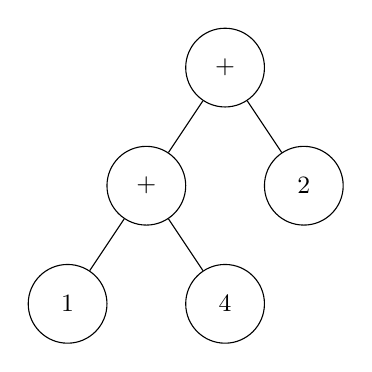
\begin{tikzpicture}[
        level distance=1.5cm,
        sibling distance=2cm,
        every node/.style={circle, draw, minimum size=10mm, font=\small},
      ]

      \node {$+$}
      child { node {$+$}
        child { node {$1$} }
        child { node {$4$} }
      }
      child { node {$2$} };

    \end{tikzpicture}
    \centering
  \end{figure}

  não incluiria nós para representar parênteses ou nós para não
  terminais. A melhor forma de representar uma AST depende da linguagem
  de programação. Em uma linguagem funcional como Haskell, é
  conveniente projetar a AST como um tipo de dados algébrico que usa um
  construtor para cada regra presente na gramática. A seguir,
  apresentamos o tipo \haskell{Exp} que representa a
  árvore de sintaxe abstrata para a gramática de expressões.

\begin{minted}{haskell}
data Exp
  = EInt Int
  | Exp :+: Exp
  | Exp :*: Exp
\end{minted}

  \subsection{Outros problemas na análise sintática}

  Algumas linguagens de programação apresentam desafios adicionais para
  a análise sintática. Por exemplo, o uso significativo de espaços em
  branco (após um hiato de várias décadas) voltou a ser comum em
  linguagens como Python, Haskell e JavaScript. Os níveis de indentação
  em Python e Haskell sinalizam implicitamente o agrupamento de
  expressões. A estratégia usual para analisar linguagens com essa
  característica é o analisador léxico inserir tokens adicionais nos
  pontos onde o nível de indentação muda. Esses tokens são conhecidos
  como tokens de indentação/desindentação. Eles podem então ser usados
  na gramática da linguagem como se fossem
  parênteses ou chaves invisíveis.

  Outro desafio são as linguagens que distinguem diferentes categorias
  de identificadores. O analisador léxico deve gerar diferentes tipos
  de tokens para diferentes tipos de identificadores. Em algumas
  linguagens, como OCaml, essa distinção não é um problema, pois a
  categoria do identificador pode ser determinada na análise léxica. No
  entanto, as linguagens C e C++ são mais difíceis de lidar. Por
  exemplo, a análise sintática correta para a declaração

\begin{minted}{cpp}
HashTable<K,V> x;
\end{minted}

  depende se \cpp{Hashtable} é o nome de uma
  classe. Se for o nome de uma variável inteira, a instrução descreve,
  na verdade, duas comparações entre quatro variáveis!

  Para gerar diferentes tipos de tokens para diferentes tipos de
  identificadores, são necessárias informações de estágios posteriores
  do compilador durante a análise léxica. Esse feedback do analisador
  léxico torna o compilador mais complexo e frágil, já que a compilação
  deixa de ser uma simples sequência linear de transformações.

  Outra técnica para lidar com análises sintáticas ambíguas é adiar o
  problema para fases posteriores do compilador, quando mais
  informações estiverem disponíveis, como a árvore sintática abstrata
  completa do programa. Essa abordagem funciona bem quando não é
  necessário resolver a ambiguidade para obter a estrutura da árvore
  sintática correta (o que não é o caso em C++, como mostra o exemplo).

  \section{Conclusão}

  Esse capítulo apresentou uma introdução à análise sintática.
  Primeiro, demonstramos por que as expressões regulares são
  insuficientes para lidar com a estrutura recursiva e balanceada das
  linguagens de programação. Através do uso de Gramáticas Livres de
  Contexto (GLCs), foi possível formalizar a sintaxe de expressões e
  resolver problemas de ambiguidade, precedência e associatividade.
  Discutimos o conceito de Árvore de Sintaxe Abstrata (AST), que serve
  como uma representação simplificada e essencial para as fases
  subsequentes de análise semântica e geração de código.

  Em seguida, apresentamos duas transformações fundamentais sobre
  gramáticas livres de contexto: a \textbf{remoção de recursão à
  esquerda}, que elimina produções que causariam loops infinitos em
  analisadores descendentes, e a \textbf{fatoração à esquerda}, que
  elimina ambiguidades de escolha entre alternativas com prefixo comum.
  Essas transformações são pré-requisitos para a construção de
  analisadores LL(1), que estudaremos em capítulos posteriores.

  Por fim, discutiu-se como desafios modernos, como a indentação
  significativa e identificadores dependentes de contexto, exigem
  estratégias sofisticadas para sua solução.
